\section{Executive Summary}
In this assignment, we need to understand how to use different techniques to get knowledge about the data we have. We can use that data to get measurements for predictions, the correlation between data points.
\newline\newline
\noindent
First, we begin analyzing the Relationship between defects and size (KLOC). 
\begin{center}
    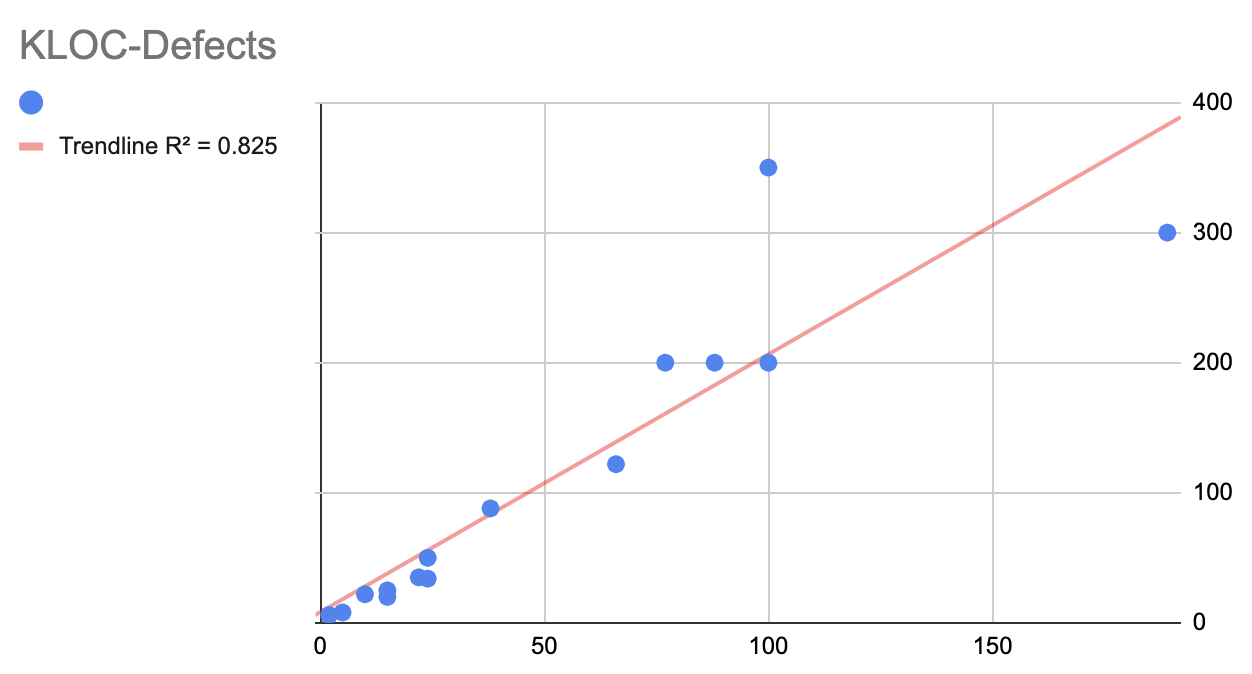
\includegraphics[scale=0.57]{scatter-plot}    
\end{center}

\noindent
We use scatter diagrams and defined KLOC in the x-axis (because they are the independent value) and defects in the y-axis (because they depend on the KLOC).
\newline\newline
\noindent
After that we calculate the trendline to know how strong is the relation ship between these 2 values, which give us a total of \textbf{0.825}.
\newline\newline
\noindent
This tells us that the relationship \textbf{KLOC - Defect} has a \textbf{very high} strength of the relationship. The more lines of code the project has the more defects.

\pagebreak
\noindent
With the following data we are going to draw a \textbf{Box and Whisker plot}

\begin{center}
    \begin{tabular}{|p{2.5cm} | c | c|}
        \hline
        Values & \textbf{KLOC} & \textbf{Defects} \\ [0.5ex] 
        \hline
        Min & 2 & 6 \\  
        \hline
        Q1 & 8 & 23.5    \\
        \hline
        Median & 24 & 50 \\
        \hline
        Q2 & 82.5 & 200  \\  
        \hline
        Maximun & 189 & 250 \\
        \hline
    \end{tabular}
\end{center}

\noindent

We get the smallest value for KLOC and Defects, then we apply those values in the \textbf{min} row, we do the same for maximum but instead of getting the smallest value we get the largest one and put it in the \textbf{maximum} row.
\newline\newline
\noindent
After we calculate the median and put it in the \textbf{median} row, we get the first quartile by using the function \textit{QUARTILE(range, 1)} and put it in the \textbf{Q1} row, and use the same function but replace de 1 for a 3 to get the second quartile, \textit{QUARTILE(range, 3)} and put the values in \textbf{Q2}.

\begin{center}
    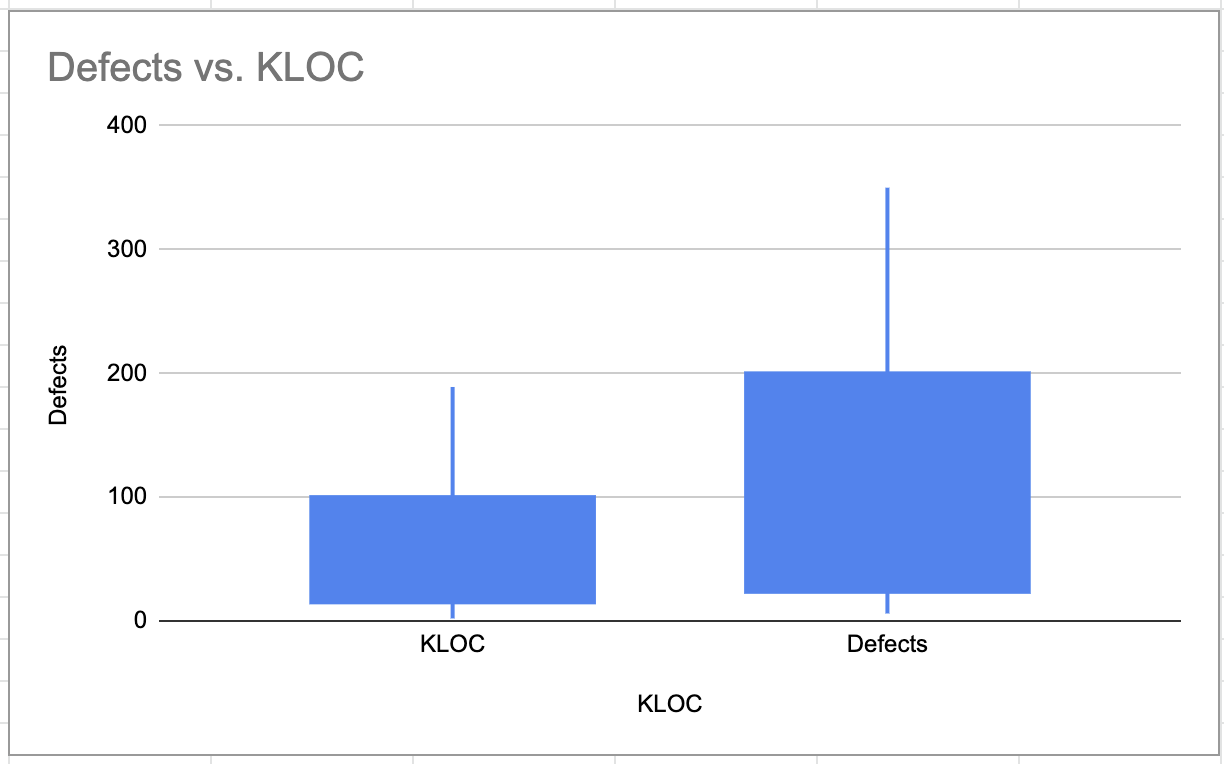
\includegraphics[scale=0.8]{box}    
\end{center}
\noindent
From this chart we can determine that amount of defects per KLOC is amount of time higher, meaning that a few KLOC could potentially create a lot of defects.

\pagebreak

\section{Observations}
\begin{itemize}
    \item In mobile there is a layout shift when you go to similar pages, instead of keeping the same size for the banners, they are different sizes on different pages.
\end{itemize}
\pagebreak

\section{Key learning}
\begin{itemize}
    \item Hello world
\end{itemize}

\pagebreak

\section{Commentary}
